\chapter{Projeto de Implementação do OpenStack no IFB}
\label{ref:implementation_project_openstack_ifb}

Todos os detalhes apresentados neste desenvolvimento foram baseados na documentação oficial do OpenStack~\citep{DocumentacaoOpenstack}. Algumas configurações específicas relacionadas às VMs foram obtidas em discussões sobre problemas registrados no \textit{\href{https://bugs.launchpad.net/openstack/}{lauchpad bugs (OpenStack)}}.

A finalidade deste capítulo é detalhar o processo de implementação do OpenStack no campus do Instituto Federal de Brasília, apresentando a arquitetura proposta, as configurações realizadas nos diferentes nós (Controller, Storage e Compute), e os ajustes necessários para atender às demandas específicas da instituição. Além disso, são abordadas estratégias de automação, criação de projetos para diferentes perfis de usuários e as considerações para futuras atualizações e migrações, garantindo a escalabilidade e a eficiência do ambiente implementado.


\section{Kolla}
Para construir nosso \textit{cluster} OpenStack, é necessário definir como o serviço será colocado em produção e como as máquinas serão distribuídas dentro do \textit{cluster}. Optamos pelo uso do \textit{\href{https://docs.openstack.org/kolla-ansible/latest/}{Kolla-Ansible}} devido à sua organização, facilidade de configuração e capacidade de automação.

O Kolla utiliza containeres Docker para executar os serviços de forma isolada, proporcionando maior controle sobre cada componente. Essa abordagem permite escalar serviços, alterar imagens, adicionar configurações específicas e realizar modificações sem impactar os demais serviços do \textit{cluster}. A utilização de containeres também facilita a manutenção e atualizações, uma vez que cada serviço opera de maneira independente.

Além disso, o Kolla-Ansible permite definir em qual nó cada serviço será executado, organizando grupos de controle que atribuem os containeres aos nós correspondentes. Por padrão, o Nó principal (\textbf{Controller}) executa todos os serviços essenciais, enquanto os demais Nós recebem serviços específicos de acordo com suas funções, como \textit{Compute} ou \textit{Storage}. No entanto, também é possível configurar qualquer Nó para executar todos os serviços, dependendo da necessidade.

O OpenStack utiliza o \textbf{HAProxy} para realizar o balanceamento de carga entre os diferentes Nós, garantindo melhor distribuição do tráfego e alta disponibilidade. Isso elimina a necessidade de configurações adicionais de balanceamento, desde que os Nós estejam na mesma rede.

O Kolla oferece diferentes versões para organizar e gerenciar as imagens Docker de forma eficiente. No nosso caso, optamos pelo lançamento mais estável disponível no momento desta pesquisa, ``ubuntu-noble''. Essa escolha foi feita porque versões mais recentes nem sempre possuem todas as imagens \textit{builded}, o que pode levar à ausência de imagens importantes, como o \textit{Cinder} executando a versão ``rocky''. Para configurar a \textit{release} desejada, basta alterar a variável \texttt{openstack\_tag} no arquivo \texttt{globals.yaml} e executar o \textit{deploy}.

No Linux, o Python é essencial para o funcionamento de serviços do sistema, e alterar pacotes ou versões globalmente pode causar problemas. Por isso, é recomendável usar ambientes virtuais para isolar dependências de projetos, evitando interferências no sistema ou em outros projetos. Ferramentas como o pyenv permitem instalar e gerenciar versões específicas do Python de forma segura, criando ambientes virtuais dedicados sem afetar a versão padrão do sistema. Essa abordagem protege o sistema operacional e mantém um ambiente de desenvolvimento consistente. Para a instalação do kolla vamos utilizar o `python venv` e dentro dele instalar os pacotes essenciais do kolla como recomendado em \textit{\href{https://docs.openstack.org/kolla-ansible/latest/user/quickstart.html}{Kolla Ansible documentation}}.

Ao final do desenvolvimento, explicaremos como organizar nosso \textit{cluster} para facilitar futuras migrações e atualizações. Como os serviços estão isolados em containeres, as atualizações tornam-se mais simples, permitindo a substituição individual de cada imagem sem impacto significativo nos demais serviços. Além disso, o Kolla garante uma retrocompatibilidade entre os containeres, tornando a troca entre versões mais estável e segura.


\section{Hardware}

O objetivo principal é aproveitar o hardware remanescente para construir uma nuvem privada, com a possibilidade de, no futuro, expandir essa infraestrutura para uma nuvem completa. Essa expansão permitiria distribuir todo o hardware disponível de forma eficiente, beneficiando diretamente os alunos do campus. Além disso, será demonstrado adiante como essa abordagem simplifica a distribuição de poder computacional e oferece maior visibilidade sobre a utilização dos recursos em cada projeto.

Para a criação de um nó (Nó) simples do OpenStack, recomenda-se uma CPU com 24 núcleos, 24 GB ou mais de memória RAM e 4 discos de 500 GB (7200 RPM)~\citep{DocumentacaoOpenstack}, conforme ilustrado na Figura \ref{fig:hardware_requirements}. Como o cluster é composto por 3 nós, esses recursos precisariam ser triplicados para atender às demandas do ambiente.

Devido às limitações do hardware disponível, essa configuração não é viável. Portanto, será criado apenas para fins de demonstração e apresentaremos a arquitetura do cluster, como deveria ser feito em servidores em produção, a forma como vamos estrutura essa arquitetura deixa simples a adição e substituição de mais nós.

\begin{figure}[htbp]
    \centering
    \caption{Requisitos de hardware recomendados para a criação de um Nó OpenStack. A figura apresenta as especificações mínimas de CPU, memória e armazenamento necessárias para um nó OpenStack simples, com recomendações para ambientes de produção.}
    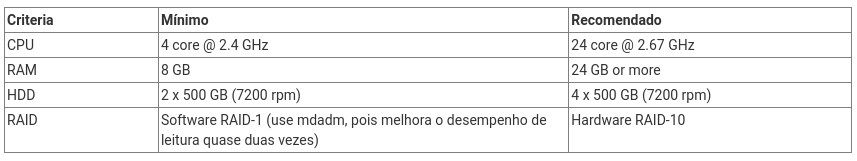
\includegraphics[width=0.9\textwidth]{images/hardware_requirements.png}
    \caption*{\textit{Fonte:} \url{https://docs.openstack.org/murano/rocky/admin/deploy_murano/prerequisites.html}.}
    \label{fig:hardware_requirements}
\end{figure}


\section{Arquitetura Geral}

Para implementar uma nuvem privada no campus do IFB, o \textit{cluster} OpenStack será composto por três nós: um nó principal (\textbf{Controller}), responsável pelos serviços essenciais, e dois nós adicionais dedicados, respectivamente, à criação de instâncias (\textit{Compute}) e ao armazenamento (\textit{Storage}). Essa divisão funcional segue o princípio de modularidade, conferindo escalabilidade e organização à arquitetura.

O \textbf{Controller} gerencia os demais nós do \textit{cluster}, centralizando a criação e administração de recursos. As configurações principais do OpenStack são definidas no arquivo \texttt{globals.yaml}, localizado em \texttt{/etc/kolla/globals.yaml}, que especifica os serviços executados, interfaces de rede e alocações de IP, incluindo o Neutron. Configurações adicionais, como a relação entre os nós, são feitas no arquivo \texttt{multinode}, encontrado em \texttt{venv/share/kolla-ansible/ansible/inventory/multinode}.

\begin{figure}[htbp]
    \centering
    \caption{Arquitetura geral do \textit{cluster} OpenStack no IFB, mostrando a distribuição dos nós: \textbf{Controller}, responsável pelos serviços essenciais; \textbf{Compute}, para criação de instâncias; e \textbf{Storage}, dedicado ao armazenamento. A figura ilustra a relação funcional e as conexões entre os componentes.}
    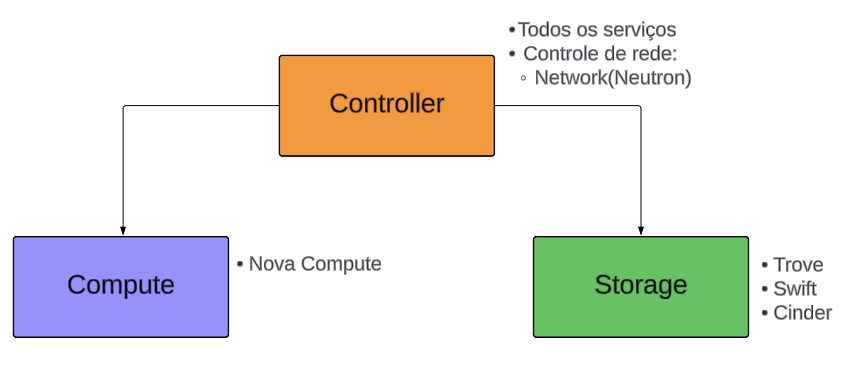
\includegraphics[width=0.7\textwidth]{images/cluster_architecture.png}
    \label{fig:cluster_architecture}
\end{figure}

Apesar de simples, essa arquitetura atende a todos os requisitos que comentamos sobre o campus, permitindo a criação de usuários, alocação de projetos e gerenciamento automatizado de recursos com agilidade. Além disso, o monitoramento detalhado possibilita tomadas de decisão informadas e a adição de recursos específicos para atender a demandas crescentes, garantindo flexibilidade e desempenho.

\section{Controller}

Devido às limitações do hardware, composto por servidores antigos com 16 GB de RAM e 120 GB de armazenamento total por nó, a configuração busca otimizar os recursos disponíveis. Essa capacidade é muito inferior à recomendada, mas é suficiente para executar o OpenStack em um ambiente de testes.

Uma limitação significativa é a ausência de discos dedicados exclusivamente a serviços de armazenamento como o \textbf{Swift} e o \textbf{Cinder}, que requerem volumes lógicos preferencialmente alocados em discos separados. No entanto, nesta configuração, todos os serviços operam em conjunto no mesmo ambiente.

\subsection{Ambiente de Teste com VMs}
Também foram realizados testes em VMs para compreender a arquitetura, sua conectividade e o gerenciamento. Esses testes se mostraram eficientes facilitando o controle e os ajustes necessários, proporcionando um ambiente flexível para experimentação. A seguir, é apresentada uma explicação simplificada sobre como essa arquitetura de teste foi configurada.

Para garantir estabilidade, as VMs foram configuradas com 18 GB de RAM, adequadas para suportar serviços críticos, como o sistema de filas. O nó \textbf{Controller} utiliza 4 vCPUs, enquanto os nós de \textit{compute} e \textit{storage} operam com 3 vCPUs cada. Apesar de ocasionais momentos de lentidão, essa configuração atende à demonstração proposta.

O \textbf{Controller} foi equipado com 120 GB de armazenamento para maior estabilidade, enquanto os demais nós utilizam 60 GB, suficientes para o propósito do teste. Em ambientes de produção, o nó de \textit{storage} demandaria uma maior capacidade de armazenamento para gerenciar grandes volumes de dados, e o nó de \textit{compute} necessitaria de mais memória RAM e processadores mais robustos para múltiplas instâncias simultâneas, a quantidade exata vai depender diretamente da quantidade de infraestrutura que será provida pelo campus.

Adicionalmente, dois discos extras foram alocados ao \textbf{Controller} para gerenciar \textit{storage}: um dedicado ao \textbf{Swift (Object Storage)} e outro ao \textbf{Cinder (Block Storage)}. A configuração desses discos é realizada no \texttt{globals.yaml}, sendo necessário criar os volumes lógicos previamente.

Embora o \textbf{Controller} gerencie serviços de armazenamento, um nó dedicado ao \textit{storage} pode ser adicionado ao \textit{cluster} para balancear a carga. O OpenStack distribui os dados automaticamente entre os nós disponíveis, permitindo escalabilidade conforme necessário, com adição eficiente de novos nós para atender ao crescimento das demandas.



\subsection{Configurações do Host OpenStack}

Como mencionado anteriormente, é fundamental compreender o papel dos volumes lógicos utilizados no \textit{cluster}, pois eles simplificam significativamente o gerenciamento de espaço. Com o uso de volumes lógicos, alterações como adicionar, remover ou modificar \textit{HDs} podem ser realizadas de forma transparente, sem a necessidade de alterar as configurações do \textit{cluster} OpenStack. Toda a manipulação ocorre diretamente nos volumes lógicos, garantindo maior flexibilidade e praticidade na administração dos recursos.

O nó \textbf{Controller} exige pelo menos duas interfaces de rede: uma para conexão interna e outra para conexão externa. No entanto, como não há uma conexão externa disponível para provisionar IPs públicos, utilizaremos às duas interfaces de forma diferente. Uma delas será dedicada ao Neutron, mas sem suporte para alocar IPs públicos diretamente às instâncias. Ainda assim, será possível utilizar o gateway padrão do \textit{switch} tendo acesso à internet e sendo possível que todos os usuários da rede interna acessem e utilizem as instâncias normalmente.

No caso da implementação em VMs, utilizaremos também duas interfaces porem configuradas para executar em modo \texttt{bridge}:
\begin{itemize}
    \item A primeira interface será configurada em modo \textit{bridge} com o host para permitir a comunicação interna.
    \item A segunda interface também será em modo \textit{bridge}, dedicada ao serviço \textbf{Neutron}, responsável por prover \textit{Network as a Service} (NaaS).
\end{itemize}

Os endereços IP estáticos para essas interfaces devem ser definidos no \texttt{netplan}. É essencial configurar IPs fixos para os nós, pois no arquivo \texttt{multinode} é necessário especificar o IP ou o DNS do nó que será utilizado nos grupos de controle. Além disso, é necessário reservar um endereço IP exclusivo na rede para o \textbf{\textit{Kolla Internal VIP Address}}, utilizado na comunicação interna entre os serviços do OpenStack. A configuração deve ser como a mostrada em Código \ref{code:globals_vip_address}.

\begin{listing}[h!]
    \noindent\fcolorbox{black}{gray!10}{%
    \parbox{\textwidth}{%
      \inputminted[]{yaml}{files/globals_vip_address.yaml}
    }%
  }  
  \caption{Exemplo de configuração do endereço VIP interno e externo do Kolla no arquivo \texttt{globals.yaml}. Essa configuração inclui a definição das interfaces de rede (\texttt{network\_interface} e \texttt{neutron\_external\_interface}) e o \texttt{kolla\_internal\_vip\_address}, que deve ser um endereço IP exclusivo e não alocado, utilizado para a comunicação interna entre os serviços do OpenStack.}
  \label{code:globals_vip_address}
\end{listing}

O parâmetro \texttt{kolla\_base\_distro} é utilizado para especificar a distribuição do sistema operacional em que os serviços do OpenStack serão executados. Essa configuração auxilia o OpenStack a determinar quais pacotes devem ser instalados e como gerenciá-los dentro do \textit{cluster}.

\subsection{Configuração de Rede}
A configuração da rede no OpenStack é um dos aspectos mais críticos para o funcionamento de um \textit{cluster}, pois garante a conectividade entre os nós e permite que as instâncias interajam com redes internas e externas. Uma rede bem configurada é essencial para a comunicação entre serviços, o acesso a recursos externos.

\subsection{Configuração de Rede Externa}
A configuração de uma rede externa no OpenStack é essencial para permitir o acesso a recursos fora do \textit{cluster} e para possibilitar a comunicação das instâncias com redes públicas ou corporativas. Esse processo inclui a definição da interface de rede física (ou virtual, no caso de VMs) responsável pela conexão externa, bem como a configuração do \textit{gateway} e do roteamento de tráfego. Após essa etapa, é necessário criar a rede externa e a sub-rede correspondente (\textit{subnet pool}), definindo a faixa de IPs públicos disponíveis, utilizando o Horizon ou a \textit{CLI}.

Antes de iniciar a configuração, os seguintes pré-requisitos devem ser atendidos:
\begin{itemize}
    \item Identificar e definir a interface de rede a ser utilizada para a conexão ao meio externo.
    \item Alocar previamente os endereços IP públicos e a máscara de rede correspondente.
    \item Configurar o \textit{gateway} padrão e validar as regras do \textit{firewall}, garantindo que o tráfego necessário esteja permitido.
\end{itemize}

No caso de testes realizados em máquinas virtuais, é necessário configurar uma interface de rede no modo \textit{bridge}. Essa interface deve ser a mesma especificada no arquivo de configuração \texttt{globals.yaml} para o Neutron. Essa configuração garante que o tráfego da interface \texttt{br-ex} seja corretamente encaminhado para a rede externa, permitindo o acesso à internet pelas instâncias. 

Além disso, independentemente da forma de \textit{deployment}, se você estiver utilizando o \textbf{OVS} para controle de rede, padrão utilizado pelo OpenStack, é crucial verificar se os parâmetros \texttt{local\_ip} e \texttt{bridge\_mappings} estão configurados corretamente no arquivo \texttt{openvswitch\_agent.ini}, como no Código \ref{code:config_openvswitch}.


\begin{listing}[h!]
    \noindent\fcolorbox{black}{gray!10}{%
    \parbox{\textwidth}{%
      \inputminted[]{ini}{files/config_openvswitch.ini}
    }%
  }  
  \caption{Configuração do arquivo \texttt{openvswitch\_agent.ini} para habilitar o suporte à rede no cluster utilizando o OpenvSwitch (\textbf{OVS}). Os parâmetros \texttt{bridge\_mappings} e \texttt{local\_ip} são essenciais para associar as redes físicas às pontes virtuais e definir o IP local do nó no \textit{cluster}.}
  \label{code:config_openvswitch}
\end{listing}

\subsection{SSH Entre os Nós}
A configuração do acesso SSH é necessária na conexão dos nós, pois permite que o host principal gerencie e execute comandos em todo o \textit{cluster}.

Para configurar o acesso SSH, é necessário criar uma chave SSH no \textbf{controller} e garantir que ele tenha acesso com permissões de \textit{root} a todos os outros nós do \textit{cluster}. Essa configuração elimina a necessidade de fornecer senhas para executar comandos com privilégios elevados, simplificando a administração e automação.

O processo envolve copiar a chave pública gerada no \textbf{controller} para cada nó utilizando o comando \texttt{ssh-copy-id}. Após isso, o usuário configurado geralmente já terá acesso como \textit{sudo}. Caso contrário, será necessário acessar o nó, editar o arquivo de permissões utilizando o comando \texttt{visudo}, e adicionar o usuário do \textbf{controller} à lista de usuários com permissões de \textit{root}. Essa configuração garante que o \textbf{controller} possa gerenciar os nós de forma segura e com o acesso necessário.


\subsection {Containers do Cluster}
Dentro do Openstack a configuração do \textbf{Docker Compose} feito pelo kolla-ansible utiliza da tag \textit{`restart.always`} isso garante que se o container sofre com algum travamento e for deletado automaticamente o docker vai tentar subir outro container igual para substituí-lo. Isso é de extrema importância para manter a saúde do \textit{cluster} e garantir que todos os serviços vão continuar habilitados.

Essa política também é seguida pelas configurações de saúde do \textit{cluster} chamado de \textit{healthcheck} garantindo que os containers sejam automaticamente recriados se forem removidos ou pararem, nesse caso até se o nó sofrer com um \textit{reboot} automaticamente, após a inicialização, ocorrerá a recriação dos containers. Essas configurações podem ser vistas dentro de `/etc/kolla/docker-compose`. Para isso funcionar o serviço do docker precisa está executando se for parado forçadamente os containers também serão destruídos.

\subsection{Docker Register}
Antes de irmos para a criação do próximo nó é necessário criar um serviço de registro no \textit{controller}, ele basicamente vai ser responsável por fornecer as imagens dos serviços para os outros nós, dessa forma garantimos a consistência das imagens em todo o \textit{cluster}. Pode ser criado mais de um registro dentro do \textit{cluster}, assim como pode ter vários \textit{controllers}. No nosso caso apenas um já resolve o problema. No \texttt{globals.yaml} deve ser adicionado as variáveis como mostrado no Código \ref{code:docker_registry_globals}.

\begin{listing}[h!]
    \noindent\fcolorbox{black}{gray!10}{%
    \parbox{\textwidth}{%
      \inputminted[]{yaml}{files/docker_registry_globals.yaml}
    }%
  }  
  \caption{Configuração do \texttt{globals.yaml} para definir o \texttt{Docker registry} interno, especificando as variáveis necessárias para que o registro forneça as imagens de forma consistente aos demais nós do cluster.}
  \label{code:docker_registry_globals}
\end{listing}


Após subir o Docker Registry e enviar as imagens para ele, é necessário alterar o arquivo \texttt{/etc/docker/daemon.json} no Docker para direcionar o \textit{pull} das imagens primeiramente ao serviço de registro configurado no \textbf{Controller}. Isso garante que, ao adicionar novos nós ao \textit{cluster}, eles busquem as imagens diretamente do registro interno, assegurando a consistência das imagens. Além disso, essa configuração facilita a propagação de novas imagens no \textit{cluster}, tornando o processo mais eficiente e controlado. Nas configurações do Docker no arquivo \texttt{deamon.json} deve se adicionar Código \ref{code:docker_insecure_registry}.


\begin{listing}[h!]
    \noindent\fcolorbox{black}{gray!10}{%
    \parbox{\textwidth}{%
      \inputminted[]{json}{files/docker_insecure_registry.json}
    }%
  }  
  \caption{Configuração do arquivo \texttt{daemon.json} para incluir o registro interno no Docker como uma rota insegura (\textit{http}), permitindo que os nós do \textit{cluster} realizem o \textit{pull} das imagens diretamente do \texttt{Docker registry} interno.}
  \label{code:docker_insecure_registry}
\end{listing}


\subsection{Configuração Multinode}
Para finalizar, é necessário ajustar o arquivo de configuração do Kolla-Ansible, chamado \textbf{multinode}, para especificar de forma clara quais serviços estão associados a cada nó do cluster. Nesta configuração, os serviços são organizados em grupos, como o \textbf{[Controler]}. No nosso caso, adicionamos o segundo nó ao grupo \textbf{[Storage]}. Essa definição no arquivo \textbf{multinode} garante que o \textbf{Controller} saiba exatamente onde cada serviço deve ser instalado e como acessar os demais nós. O arquivo \textbf{multinode} deve seguir o formato ilustrado no Código \ref{code:config_multinode}.

\begin{listing}[h!]
    \noindent\fcolorbox{black}{gray!10}{%
    \parbox{\textwidth}{%
      \inputminted[]{ini}{files/config_multinode.ini}
    }%
  }  
  \caption{Configuração do arquivo multinode separando os grupos de controle entre os nós.}
  \label{code:config_multinode}
\end{listing}

Caso seja necessário criar variáveis de ambiente ou configurar caminhos padrões do openstack, como o caminho do \textbf{python} que será utilizado, pode-se alterar o arquivo \textbf{ansible.cfg} naturalmente encontrado em \texttt{`~/ansible/`}, caso não tenha sido criado pelo \textbf{deployment} do \textit{multinode}, não tem problema criar o arquivo direto em \texttt{`~/.ansible.cfg`}. 

Para verificar se o OpenStack está utilizando o arquivo de configuração correto, pode-se executar o comando \texttt{`ansible --version`}:

\section{Segundo Nó (Storage)}

Este nó será dedicado exclusivamente ao armazenamento, utilizando os serviços \textbf{Cinder} e \textbf{Swift}, cada um alocado em \textit{volume groups} separados. Inicialmente, cada \textit{volume group} (\texttt{cinder-volumes} e \texttt{swift-volumes}) será configurado com um único disco. Essa abordagem oferece flexibilidade para futuras expansões, permitindo adicionar novos discos ao \textit{volume group} sem complexidade significativa.

A criação inicial dos \textit{volume groups} é realizada manualmente no \textbf{Controller}, que também executa todos os serviços essenciais. Dessa forma, é necessário alocar previamente os discos destinados ao \textbf{Swift} e ao \textbf{Cinder} no \textbf{Controller} antes de configurar o nó de \textit{storage}. Após essa etapa, é possível automatizar a criação de volumes e a configuração dos discos, reduzindo a necessidade de intervenção manual nos nós. Caso novos discos sejam adicionados após a implantação inicial, eles podem ser incluídos manualmente nos \textit{volume groups} do nó de \textit{storage} de forma simples e eficiente.

Uma vez configurado o \textbf{Controller}, é essencial garantir que ele tenha acesso ao nó de \textit{storage}. Isso requer a configuração das chaves SSH para permitir o acesso seguro e direto do \textbf{Controller} ao nó de \textit{storage}, eliminando a necessidade de autenticação manual. Além disso, é necessário atualizar o arquivo de inventário \texttt{/etc/kolla/inventory/multinode} com o endereço IP ou DNS do nó de \textit{storage}, garantindo que os serviços do OpenStack possam localizá-lo corretamente.

Com o nó de \textit{storage} configurado, o \textbf{Cinder} gerenciará volumes para instâncias e o \textbf{Swift} será responsável pelo armazenamento de objetos, permitindo que o \textit{cluster} atenda a diferentes demandas de armazenamento de maneira eficiente e escalável.


\section{Terceiro Nó (Compute)}

Este nó será dedicado exclusivamente à criação de máquinas virtuais (\textit{instances}), desempenhando o papel equivalente ao EC2 em provedores de nuvem pública. Ele utilizará os recursos alocados, como CPU, memória e armazenamento local, para provisionar máquinas virtuais com base nos \textit{flavors} definidos pelo usuário da organização.

Os \textit{flavors} representam as especificações das máquinas virtuais, como quantidade de CPUs, memória RAM e tamanho do disco. Esses recursos são consumidos diretamente do nó \textbf{Compute}, que é responsável por executar as instâncias e garantir sua performance, isolação e conectividade.

A configuração do nó \textbf{Compute} é realizada pelo Kolla-Ansible, utilizando o arquivo de inventário \texttt{/etc/kolla/inventory/multinode}. Neste arquivo, o nó \textbf{Compute} deve ser listado sob o grupo \textbf{[compute]} para que os serviços necessários, como o \textit{Nova Compute}, sejam implantados corretamente. Além disso, o \textbf{Controller} gerencia as tarefas administrativas relacionadas à criação, inicialização e destruição das máquinas virtuais, enquanto o nó \textbf{Compute} executa as operações físicas.

A comunicação entre o \textbf{Controller} e o nó \textbf{Compute} é feita de forma segura e direta. Seguindo a mesma ideia do outro nó, precisamos configurar a chave SSH e adicionar o DNS ou IP no arquivo \textbf{multinode}

Após a implantação inicial, o nó \textbf{Compute} estará pronto para receber solicitações de criação de máquinas virtuais. Ele será responsável por alocar os recursos conforme especificado nos \textit{flavors}, garantindo a escalabilidade e eficiência do \textit{cluster}. Caso novos nós \textbf{Compute} sejam adicionados ao \textit{cluster}, o balanceamento de carga entre os nós será automaticamente gerenciado pelo OpenStack, otimizando o uso de recursos.


\section{\textit{Deploy} da Aplicação}
Após configurar a rede e os arquivos mencionados, o \textit{deploy} dos serviços pode ser realizado. Esse processo cria múltiplos containeres que executam os serviços padrão do OpenStack, conforme ilustrado na Figura \ref{fig:controller_containers}. O acesso ao painel do OpenStack (\textbf{Horizon}) pode ser feito por meio do endereço \texttt{http://kolla\_internal\_vip\_address/dashboard}. A partir desse painel, é possível configurar todos os serviços de IaaS. Detalhes adicionais sobre a configuração dos serviços serão apresentados nas próximas seções.


\begin{figure}[htbp]
    \centering
    \caption{Containers de base do serviço OpenStack executando no nó principal do \textit{cluster} após efetuar o \textit{deploy} com o Kolla-ansible, mostrando de estão saudáveis e quando foram iniciados}
    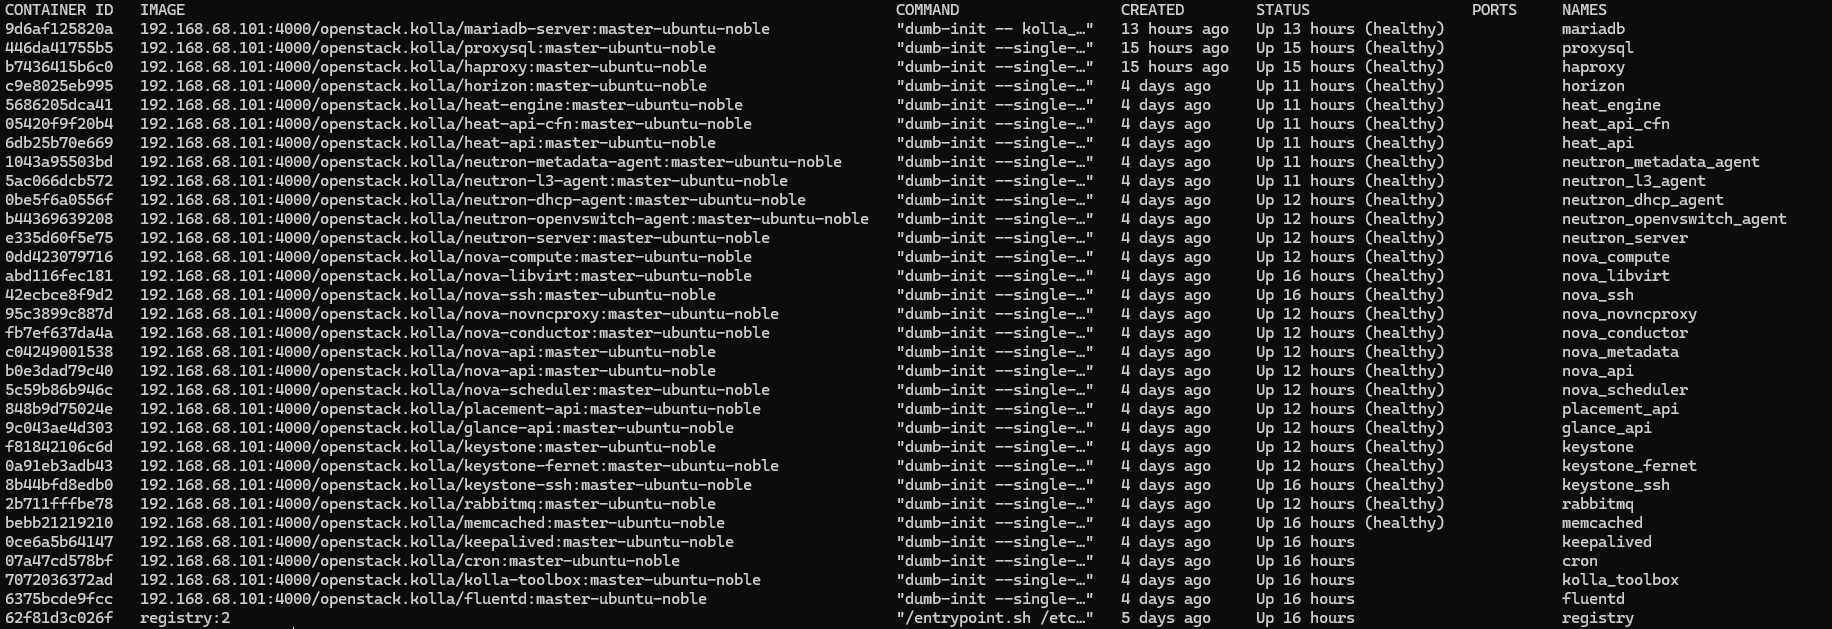
\includegraphics[width=1.0\textwidth]{images/controller_containers.png}
    \caption{Imagem retirada do terminal do nó principal do cluster}
    \label{fig:controller_containers}
\end{figure}

Os containeres exibidos, ou a maioria deles, devem estar visíveis em todos os nós do \textit{cluster}. Cada container possui a marcação \textit{health}, indicando que está em execução sem erros detectados.

\section{Por Dentro do OpenStack}
Após configurado o \textit{cluster}, é fundamental entender como o OpenStack organiza e gerenciar seus recursos. O OpenStack funciona por meio de \textbf{projetos}, que podem conter diversos \textbf{usuários}, e cada usuário tem permissões específicas definidas pelas \textit{roles}. 

A seguir, exploraremos os principais conceitos e configurações relacionados aos projetos, usuários, políticas de acesso, cotas e rede, detalhando suas funcionalidades e como interagem no ecossistema OpenStack, todos os comandos mostrados podem ser feitos direto pelo Horizon.

\subsection{OpenStack-Client}
Para utilizar a maioria dos comandos descritos nesta seção, é necessário instalar o pacote \texttt{python-openstackclient}. Isso pode ser feito utilizando o gerenciador de pacotes \texttt{pip}. Após a instalação, você deve realizar o \textit{login} configurando as variáveis de ambiente listadas abaixo.

Por padrão, as únicas alterações necessárias serão no valor de \texttt{VIP\_IP} (o endereço IP configurado) e na senha gerada automaticamente. O endereço IP pode ser consultado no arquivo \texttt{globals.yaml}, enquanto a senha pode ser obtida utilizando o comando da Figura~\ref{code:grep_password}.

\begin{listing}[h!]
    \noindent\fcolorbox{black}{gray!10}{%
    \parbox{\textwidth}{%
      \inputminted[]{sh}{files/grep_password.sh}
    }%
  }  
  \caption{Comando utilizado para recuperar a senha gerada automaticamente para a conta \texttt{admin} no arquivo de configuração do Kolla (\texttt{passwords.yml}). Essa senha será utilizada para configurar o acesso ao OpenStack.}
  \label{code:grep_password}
\end{listing}

Após obter essas informações, é possível criar o arquivo \texttt{admin\_variables.sh}, que conterá as variáveis de ambiente necessárias para acessar o \textit{admin}. Após criar esse arquivo com as variáveis demonstradas na Figura~\ref{code:source_admin}, basta executá-lo com o comando \texttt{source admin\_variables.sh}

\begin{listing}[h!]
    \noindent\fcolorbox{black}{gray!10}{%
    \parbox{\textwidth}{%
      \inputminted[]{sh}{files/source_admin.sh}
    }%
  }  
  \caption{Exemplo de configuração das variáveis de ambiente necessárias para acessar o \texttt{admin} do OpenStack utilizando o Terminal. Inclui definições do endpoint (\texttt{OS\_AUTH\_URL}), credenciais de autenticação, e outros parâmetros essenciais.}
  \label{code:source_admin}
\end{listing}

\subsection{Projetos}
Os projetos (também chamados de \textit{tenants}) agrupam recursos como instâncias, redes e volumes. Cada projeto possui isolamento de recursos, evitando interferência de um projeto sobre outro. Além disso, é possível definir cotas para limitar o uso de instâncias, redes e outros recursos. Cada projeto pode ter usuários com papéis bem definidos, garantindo um controle de acesso eficaz.

O OpenStack também permite personalizar quais serviços um projeto pode acessar, como \textit{Swift}, \textit{Glance}, entre outros. Na figura \ref{fig:openstack_projects}, é exibida a interface do \textit{dashboard} Horizon, onde podem ser realizadas as configurações relacionadas a projetos, incluindo sua criação e atribuição de permissões.

\begin{figure}[htbp]
    \centering
    \caption{Interface do Horizon mostrando a configuração e gerenciamento de projetos, local onde também é configurado todos os detalhes relacionados aos projetos.}
    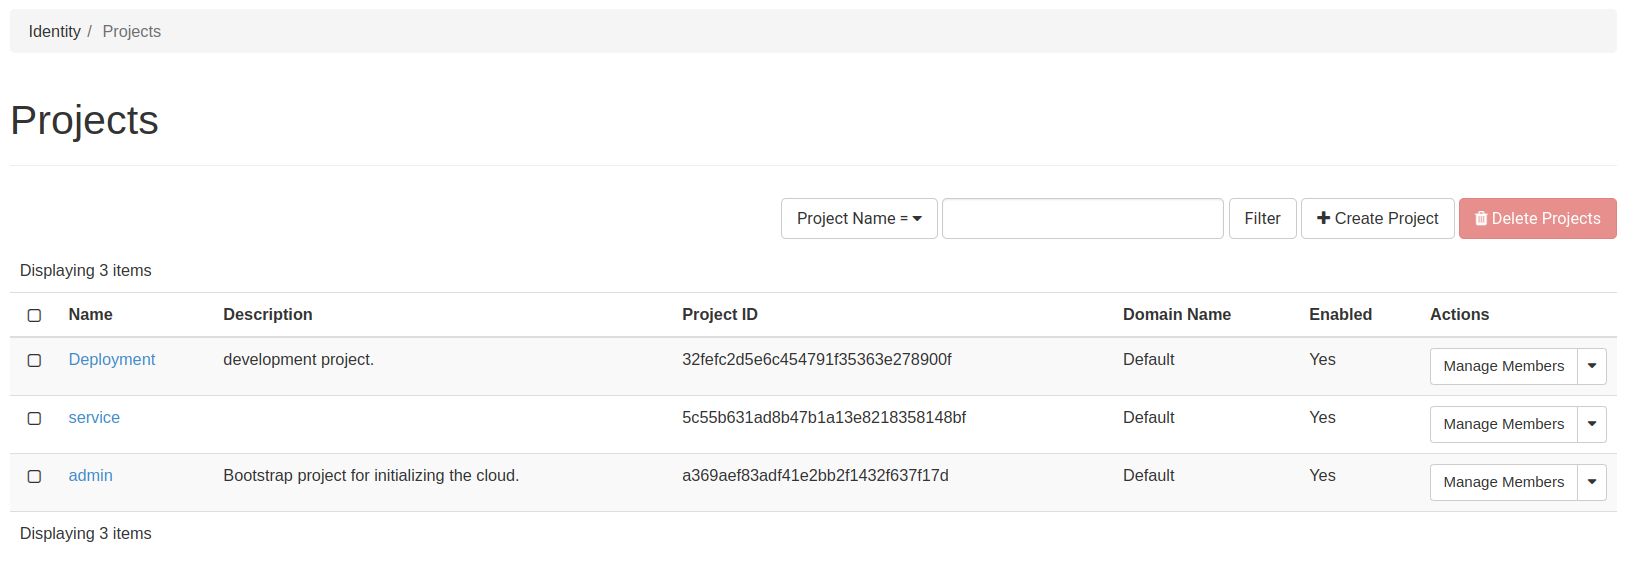
\includegraphics[width=0.9\textwidth]{images/openstack_projects.png}
    \caption*{Fonte: \textit{Dashboard} Horizon do OpenStack.}
    \label{fig:openstack_projects}
\end{figure}

Dentro dos projetos utilizamos cotas. As cotas delimitam o número de recursos que cada projeto pode consumir, como instâncias, volumes e redes. Embora sejam úteis para evitar o uso abusivo de recursos, o OpenStack não garante previamente que o \textit{cluster} tenha a capacidade de suprir todas as cotas aprovadas. Caso um projeto tente criar recursos além da capacidade disponível no \textit{cluster}, erros de criação podem ocorrer, e nós sobrecarregados podem apresentar \textit{reboots} inesperados.

\subsection{Usuários}
Os usuários são entidades autenticadas pelo serviço \textbf{Keystone}, que gerencia identidades e permissões. Eles podem ser criados tanto pela interface de linha de comando (CLI) quanto pela interface gráfica (Horizon). Cada usuário está associado a um ou mais projetos, com \textit{roles} específicas que definem suas permissões no ambiente.

O Keystone oferece suporte a diferentes métodos de autenticação, como LDAP ou banco de dados interno, permitindo integração com sistemas externos. Na figura \ref{fig:openstack_users}, é mostrado como usuários e contas de serviço são configurados de forma similar, diferenciando-se apenas pelas políticas de segurança atribuídas.

\begin{figure}[htbp]
    \centering
    \caption{Interface do Horizon mostrando usuários e contas de serviço configurados pelo Keystone.}
    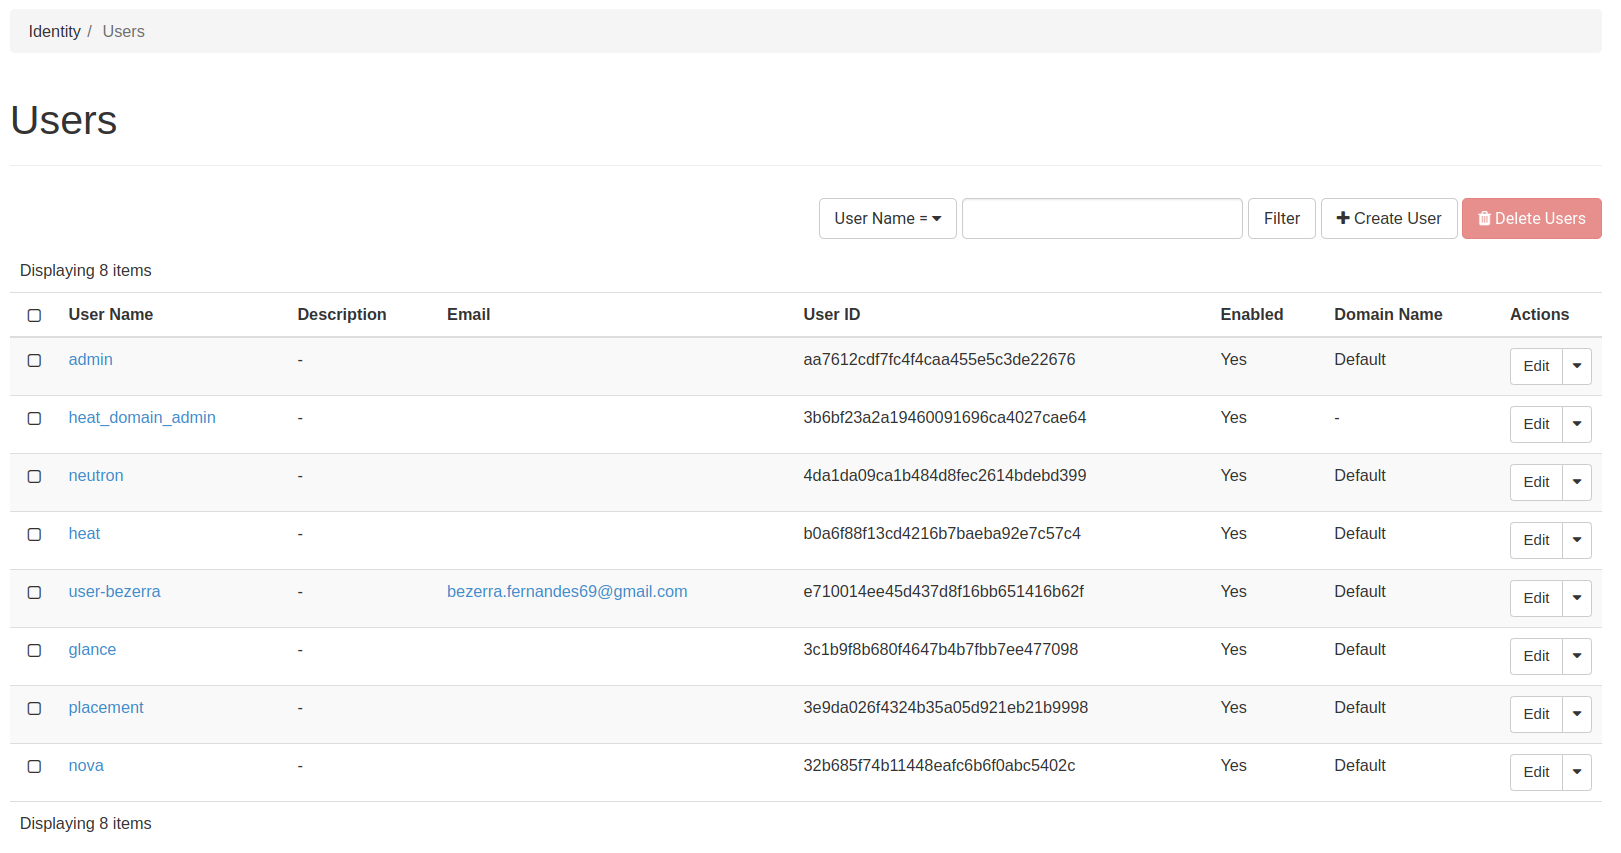
\includegraphics[width=0.9\textwidth]{images/openstack_users.png}
    \caption*{Fonte: \textit{Dashboard} Horizon do OpenStack.}
    \label{fig:openstack_users}
\end{figure}

\subsection{Políticas de Acesso para Serviços e Usuários}
As políticas de acesso, definidas em arquivos de configuração (JSON ou YAML), determinam quais operações cada \textit{role} pode executar nos serviços, como Nova, Neutron e Cinder. Isso viabiliza um controle granular, permitindo personalizar ações como criação de instâncias e gerenciamento de redes.

Em implantações como Kolla-Ansible, esses arquivos podem ser gerenciados centralmente para simplificar a administração. Na figura \ref{fig:openstack_roles}, são mostradas as \textit{roles} padrões criadas pelo OpenStack para contas de serviço.

\begin{figure}[htbp]
    \centering
    \caption{Interface do Horizon mostrando as \textit{roles} padrões do OpenStack para controle de contas de serviço.}
    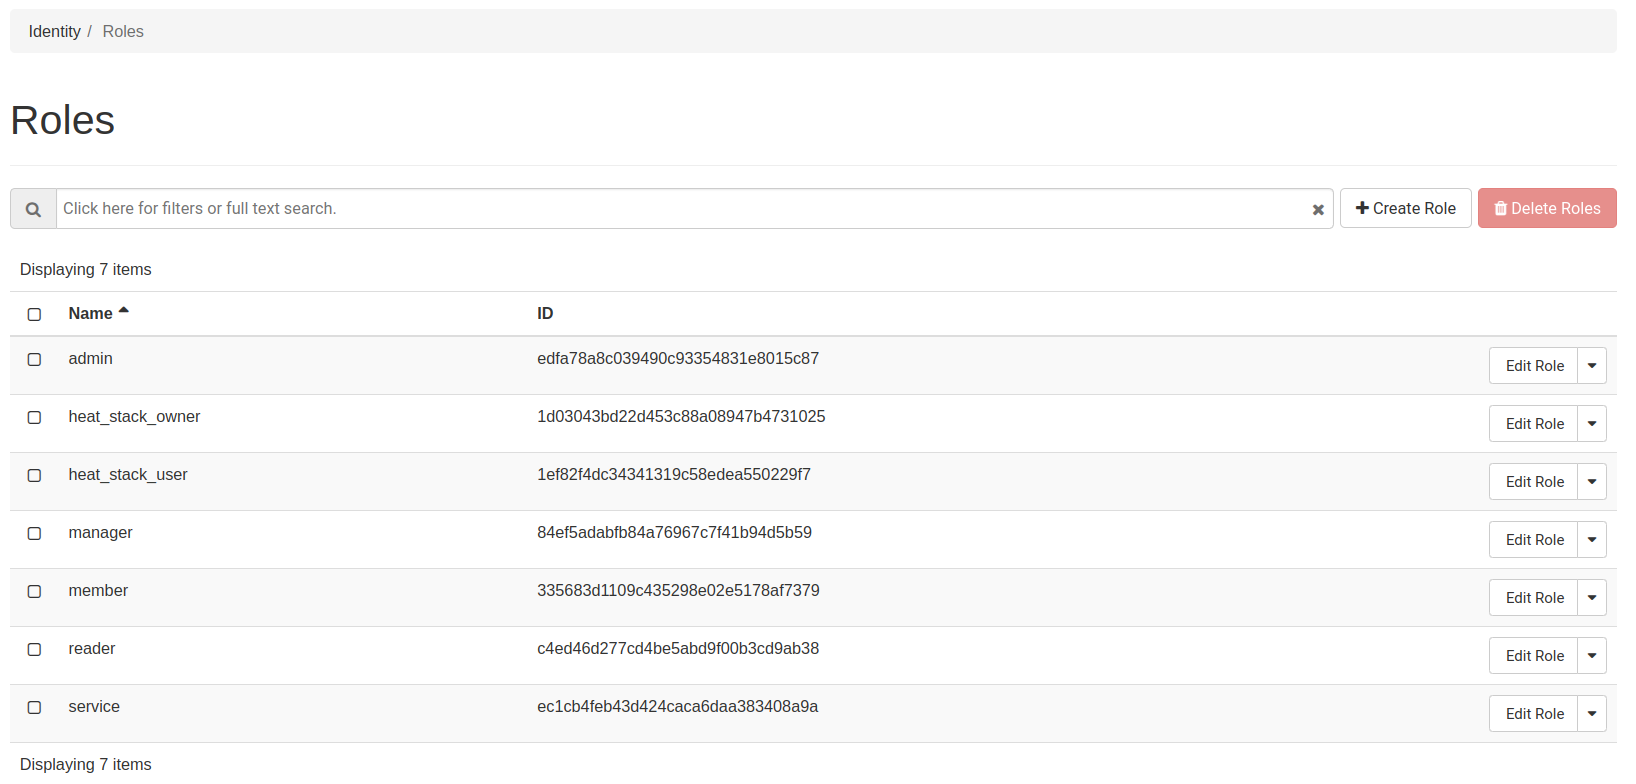
\includegraphics[width=0.9\textwidth]{images/openstack_roles.png}
    \caption*{Fonte: \textit{Dashboard} Horizon do OpenStack.}
    \label{fig:openstack_roles}
\end{figure}

\subsection{Rede}
O serviço \textbf{Neutron} gerencia a criação de redes e \textit{subnets} virtuais (ou VPCs), onde se definem regras de firewall, roteamento e conexões entre instâncias. Cada projeto pode manter suas próprias redes isoladas, garantindo segurança e organização.

A visualização da topologia de rede no Horizon (ou via \textit{CLI}) exibe como cada elemento (instâncias, roteadores e sub-redes) está interligado, ajudando a identificar rotas e possíveis pontos de falha. Após as configurações iniciais, é possível criar uma rede externa utilizando os comandos direto no terminal. No Código \ref{code:command_external_network} criamos a \textit{network} externa e definimos uma \textit{subnet} para alocar IPs no intervalo especificado em \textbf{--allocation-pool}, além de configurarmos o \textit{gateway} de saída.

\begin{listing}[h!]
    \noindent\fcolorbox{black}{gray!10}{%
    \parbox{\textwidth}{%
      \inputminted[]{sh}{files/command_external_network.sh}
    }%
  }  
  \caption{Comandos para criar uma rede externa no OpenStack. A configuração define o tipo de rede (\texttt{flat}), associa a rede ao provedor físico (\texttt{physnet1}), e configura uma sub-rede com intervalo de endereços alocados, gateway e desativação do DHCP.}
  \label{code:command_external_network}
\end{listing}


Também criamos uma rede interna Código \ref{code:command_internal_network}, que será utilizada pelas instâncias. Enquanto a rede externa é compartilhada entre projetos, as redes internas são isoladas para cada projeto, sendo criadas a partir de contas administradoras de projetos.

\begin{listing}[h!]
    \noindent\fcolorbox{black}{gray!10}{%
    \parbox{\textwidth}{%
      \inputminted[]{sh}{files/command_internal_network.sh}
    }%
  }  
  \caption{Comandos para criar uma rede interna no OpenStack. Redes internas são isoladas por projeto e utilizadas pelas instâncias. A configuração inclui a criação da rede e de uma sub-rede associada, com as definições de faixa de IPs, gateway e outras propriedades específicas.}
  \label{code:command_internal_network}
\end{listing}

Para verificar se as conexões foram configuradas corretamente, podemos acessar a área \textit{Network Topology}. Essa seção apresenta uma visualização gráfica de como a \textit{Network} está estruturada, permitindo identificar as conexões entre instâncias, roteadores e sub-redes. A figura \ref{fig:network_topology} ilustra essa visualização dentro do \textit{dashboard} Horizon.

\begin{figure}[htbp]
    \centering
    \caption{Visualização da topologia de rede no \textit{dashboard} Horizon, mostrando as conexões entre instâncias, roteadores e sub-redes.}
    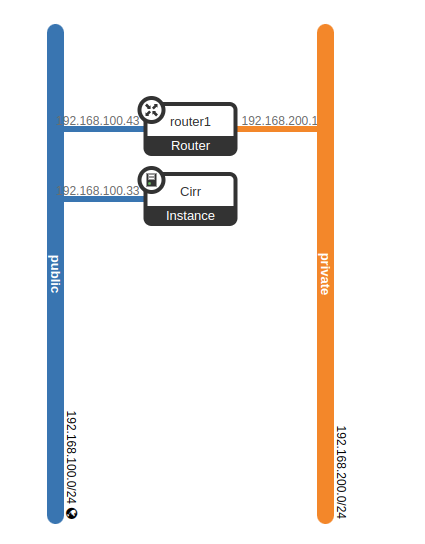
\includegraphics[width=0.5\textwidth]{images/network_topology.png}
    \caption*{Fonte: \textit{Dashboard} Horizon do OpenStack.}
    \label{fig:network_topology}
\end{figure}

\subsection{Arquitetura de Separação de Recursos para o Campus}

O OpenStack oferece diversas formas de organizar e separar projetos e usuários para atender a diferentes necessidades. No contexto de uma instituição de ensino superior, como um campus universitário, é comum a necessidade de segmentar recursos entre departamentos, e dentro desses, entre seus respectivos usuários. Uma abordagem eficiente para essa finalidade é a utilização da \href{https://wiki.openstack.org/wiki/HierarchicalMultitenancy}{\textit{Hierarchical Multitenancy}}.

Essa arquitetura permite a criação de uma hierarquia de projetos, em que subprojetos são vinculados a um projeto principal. Cada projeto principal pode representar um departamento, como Engenharia, Ciências da Computação ou Administração, enquanto os subprojetos podem ser utilizados para atividades específicas, como Trabalhos de Conclusão de Curso (TCCs), pesquisas acadêmicas ou laboratórios de ensino. 

A utilização dessa arquitetura torna-se ainda mais poderosa quando combinada com os templates do Heat. Esses templates permitem a criação automatizada de todos os componentes necessários para iniciar uma nova pesquisa ou atividade, otimizando o provisionamento de recursos e reduzindo o esforço operacional. A seguir, serão apresentados detalhes sobre os templates e suas aplicações práticas.

\subsection{Debug e Resolução de Problemas}
Devido à complexidade e constante desenvolvimento do OpenStack, erros são situações frequentes e podem exigir diferentes abordagens de depuração. A análise inicial deve sempre incluir a verificação dos arquivos de log, geralmente localizados em \textbf{/var/log/kolla/}, que fornecem informações detalhadas sobre o comportamento dos serviços e possíveis falhas. Adicionalmente, habilitar o modo de depuração nos serviços pode facilitar a identificação de problemas. Isso pode ser feito configurando a variável \texttt{DEBUG=True} no arquivo de configuração do serviço em questão.

Quando o problema envolve um erro mais profundo, como falhas em componentes do código, recomenda-se o uso do \textbf{DevStack}. O DevStack é uma ferramenta leve e altamente configurável, ideal para criar um ambiente de desenvolvimento que replica uma instalação do OpenStack em um único nó. Ele permite a execução de serviços do OpenStack em modo debug, facilitando o acesso a logs detalhados e a inserção de pontos de interrupção no código. Esse ambiente é ideal para testar alterações e investigar problemas sem afetar a instalação principal.

Para realizar uma depuração interativa com o DevStack, pode-se utilizar o depurador \textit{pdb} do Python. Insere-se a seguinte linha no código no ponto onde deseja interromper a execução: \texttt{import pdb; pdb.set\_trace()}.

Após ajustar o código, basta reiniciar o serviço no ambiente DevStack para realizar a análise interativa. Essa abordagem é vantajosa, pois permite isolar problemas e testar soluções de forma controlada antes de aplicá-las em um ambiente de produção.

Embora a maioria dos erros possa ser resolvida ajustando configurações ou corrigindo permissões, erros de código requerem conhecimento aprofundado sobre o funcionamento interno dos serviços do OpenStack e suas interações. Nesses casos, o uso do DevStack como ambiente de desenvolvimento é altamente recomendado, pois proporciona flexibilidade e controle total sobre os serviços e suas dependências.

\section{Migração e Atualizações Futuras}

No contexto de software, atualizações e correções de erros são lançadas regularmente, e o OpenStack não é uma exceção. É fundamental manter o ambiente atualizado para aproveitar novos recursos (\textit{features}) e melhorias de desempenho, além de corrigir vulnerabilidades de segurança. Antes de realizar qualquer atualização, é de extrema importância garantir que todos os backups necessários estejam disponíveis, permitindo a restauração do sistema em caso de falhas.

\subsection{Atualização de containeres}

Como mencionado anteriormente, o Kolla-Ansible isola os serviços do OpenStack em containeres Docker. Essa arquitetura permite atualizar os containeres de forma individual. No entanto, para garantir que todos os serviços sejam devidamente sincronizados, se comuniquem corretamente e, quando necessário, sejam reconfigurados automaticamente, recomenda-se realizar uma atualização completa utilizando como no Código \ref{code:update_kolla}:

\begin{listing}[h!]
    \noindent\fcolorbox{black}{gray!10}{%
    \parbox{\textwidth}{%
      \inputminted[]{sh}{files/update_kolla.sh}
    }%
  }  
  \caption{Comando para atualizar todos os serviços do OpenStack gerenciados pelo Kolla-Ansible. Essa abordagem garante que os containeres sejam sincronizados, configurados corretamente e reconfigurados automaticamente quando necessário.}
  \label{code:update_kolla}
\end{listing}

Esse procedimento garante que os containeres sejam atualizados para as versões mais recentes das imagens, aplicando automaticamente quaisquer modificações *necessárias nas configurações e garantindo a continuidade dos serviços.

Em alguns casos, quando são lançadas novas \textit{features} ou alterações significativas nas configurações, é necessário atualizar o arquivo \texttt{globals.yaml}. Esse arquivo atualizado pode ser encontrado no diretório de exemplos \texttt{../kolla-ansible/etc\_examples/kolla/*}. Após obter o novo arquivo, é necessário incorporar manualmente as configurações existentes para preservar a compatibilidade com o ambiente atual.


\section{Análise do Cluster}

Com os três nós configurados e operacionais, utilizamos serviços nativos do OpenStack para realizar a análise do cluster. Os serviços utilizados incluem:

\begin{itemize}
    \item \textbf{Gnocchi}: Responsável por coletar e armazenar métricas relacionadas ao desempenho e utilização do cluster, como uso de CPU, memória e armazenamento.
    \item \textbf{Aodh}: Utilizado para a configuração de alarmes. Este serviço nos permite definir ações automatizadas caso ocorra alguma falha.
    \item \textbf{Panko}: Registro e armazenamento de logs de eventos, mostrando exatamente o que foi feito e por qual pessoa.
    \item \textbf{Ceilometer}: Um dos principais serviços do OpenStack para medição de dados de uso. Ele fornece uma visão abrangente dos recursos consumidos, contribuindo para relatórios detalhados e para a gestão eficiente do cluster.
\end{itemize}

A integração desses serviços permite não apenas monitorar o desempenho e a utilização do \textit{cluster}, mas também detectar anomalias e registrar eventos críticos. Essa abordagem facilita a manutenção preventiva e corretiva no ambiente OpenStack.

Além disso, o \textbf{Ceilometer} permite integração com outros serviços de monitoramento amplamente utilizados, como o Grafana. Essa conexão possibilita a criação de \textit{dashboards} personalizados para visualizar métricas em tempo real, identificar tendências de uso e acompanhar o desempenho do cluster de maneira gráfica e centralizada. 

Por fim, a análise do \textit{cluster} é um passo essencial para garantir que a infraestrutura opere com alta disponibilidade, desempenho consistente e segurança, características fundamentais para atender às demandas de um ambiente acadêmico e administrativo.

\section{Implementação e Utilização de Recursos}
O Heat é o serviço de orquestração do OpenStack que permite automatizar o gerenciamento de infraestrutura por meio de templates declarativos escritos em YAML, naturalmente esse tipo de serviço é chamado de IaC  \textit{(Infraestructure as Code)}. Com ele, você pode definir, provisionar e gerenciar recursos, como instâncias, volumes, redes e até aplicações inteiras, de forma padronizada e repetível. Esse serviço é especialmente útil para configurar ambientes de trabalho para novos estudantes, permitindo que iniciem projetos com rapidez e eficiência. Além disso, o mesmo template pode ser facilmente ajustado para adicionar mais recursos, conforme a necessidade do projeto.

Os próprios alunos também podem utilizar templates do Heat para gerenciar a infraestrutura de seus projetos. Isso facilita a demonstração de quais recursos foram utilizados e como o ambiente pode ser replicado de forma simples e eficiente. Essa abordagem promove organização e consistência no uso dos recursos de infraestrutura, otimizando o aprendizado e a colaboração em projetos acadêmicos.

\subsection{Configuração para a utilização de IaC}
É possível que o serviço Heat não tenha permissões diretas para acessar e manipular o \textit{cluster}. Para contornar essa limitação, normalmente criamos um arquivo de configuração específico para o Heat em \texttt{/etc/kolla/config/heat.conf}, utilizando a configuração como mostrado no Código \ref{code:heat_configuration}.

É necessário manter esses arquivos de configuração devidamente protegidos, pois eles geralmente contêm credenciais sensíveis. Essa prática deve ser aplicada a todos os arquivos localizados em \texttt{/etc/kolla/}, garantindo a segurança do ambiente e prevenindo acessos não autorizados.


\begin{listing}[h!]
    \noindent\fcolorbox{black}{gray!10}{%
    \parbox{\textwidth}{%
      \inputminted[]{sh}{files/heat_configuration.conf}
    }%
  }  
  \caption{Exemplo de configuração do arquivo \texttt{heat.conf}, localizado em \texttt{/etc/kolla/config/}. Esse arquivo define as permissões e parâmetros necessários para o serviço Heat gerenciar a infraestrutura no \textit{cluster}.}
  \label{code:heat_configuration}
\end{listing}


\subsection{Criação de Instâncias para Alunos em Sala de Aula}

Uma aplicação prática do \textit{cluster} em um ambiente acadêmico é sua integração com as atividades em sala de aula. Considere o seguinte cenário: você está ministrando uma aula sobre processamento de imagens e deseja disponibilizar uma instância para cada aluno. Essas instâncias podem ser configuradas previamente com um ambiente virtual e todos os pacotes necessários do python já instalados, garantindo que os alunos possam se concentrar exclusivamente nos objetivos da aula.

Para alcançar esse objetivo, é possível utilizar um único template do Heat. Aplicando o conceito de \texttt{HierarchicalMultitenancy}, criamos um subprojeto denominado \texttt{aula-proc-dig} dentro do projeto principal. Nesse subprojeto, as instâncias dos alunos serão provisionadas de forma organizada Código \ref{code:template_heat_one}.

\begin{listing}[h!]
    \noindent\fcolorbox{black}{gray!10}{%
    \parbox{\textwidth}{%
      \inputminted[]{yaml}{files/template_heat_one.yaml}
    }%
  }  
  \caption{Exemplo de template Heat para provisionamento automatizado de instâncias no subprojeto \texttt{aula-proc-dig}, configuradas para atividades de processamento de imagens.}
  \label{code:template_heat_one}
\end{listing}

\newpage

\subsection{Criação de Projetos para Alunos de Pesquisa}

Para atender alunos que estão iniciando projetos de pesquisa, como CNPq ou Trabalhos de Conclusão de Curso (TCC), é possível criar um template dedicado. Também seguindo o conceito de \texttt{HierarchicalMultitenancy}, podemos provisionar uma rede e uma instância isolada para cada aluno, permitindo que eles configurem o ambiente de acordo com suas necessidades específicas. Além disso, essa abordagem facilita a escalabilidade, possibilitando a alocação de recursos adicionais de maneira ágil e controlada, caso seja necessário Código \ref{code:template_heat_two_part1}.

\begin{listing}[h!]
    \noindent\fcolorbox{black}{gray!10}{%
    \parbox{\textwidth}{%
      \inputminted[]{yaml}{files/template_heat_two_part1.yaml}
    }%
  }  
  \caption{Parte 1: Exemplo de template Heat para provisionamento de projetos individuais de pesquisa, incluindo uma rede e uma instância configurável, com suporte à escalabilidade de recursos, continuação em Código \ref{code:template_heat_two_part2}.}
  \label{code:template_heat_two_part1}
\end{listing}

\begin{listing}[h!]
  \noindent\fcolorbox{black}{gray!10}{%
  \parbox{\textwidth}{%
    \inputminted[firstnumber=26]{yaml}{files/template_heat_two_part2.yaml}
  }%
}  
\caption{Parte 2: Criação dos recursos do necessário para rodar as instâncias com a imagem escolhida em Código \ref{code:template_heat_two_part1}.}
\label{code:template_heat_two_part2}
\end{listing}

Esses templates foram projetados para atender às necessidades específicas dos alunos em atividades acadêmicas, mas a abordagem é flexível e pode ser adaptada para qualquer membro do campus que necessite de infraestrutura computacional. Professores, pesquisadores e equipes administrativas podem solicitar recursos personalizados, como instâncias, redes ou ambientes configurados, que serão provisionados de forma automatizada e organizada por meio de templates do Heat.